\documentclass[a4paper, titlepage]{livret} % classe spéciale rapport : livret

\usepackage[utf8]{inputenc} % accents
\usepackage[T1]{fontenc} % caractères français
\usepackage{geometry} % marges
\usepackage[francais]{babel} % langue
\usepackage{graphicx} % images
\usepackage{verbatim} % texte préformaté
\usepackage{listings} % code source
\usepackage[framed,numbered,autolinebreaks,useliterate]{mcode} % code source
\usepackage{listingsutf8} % code source accents
\usepackage[final]{pdfpages} % inclusion de pdf
\usepackage{url} % utilisation des url
\usepackage{caption} % nom des tableaux
\usepackage{amsmath} % maths
\usepackage{amsfonts, bbm} % fonts maths
\usepackage{algorithmeUTF8} % algorithmique

\graphicspath{{img/}} % chemin des illustrations

\title{Projet d'algorithmique} % titre
\author{Elliot Sisteron & Antoni Markovski} % auteur

\pagestyle{headings} % rappel discret (en haut à gauche)

\begin{document} % début du document

	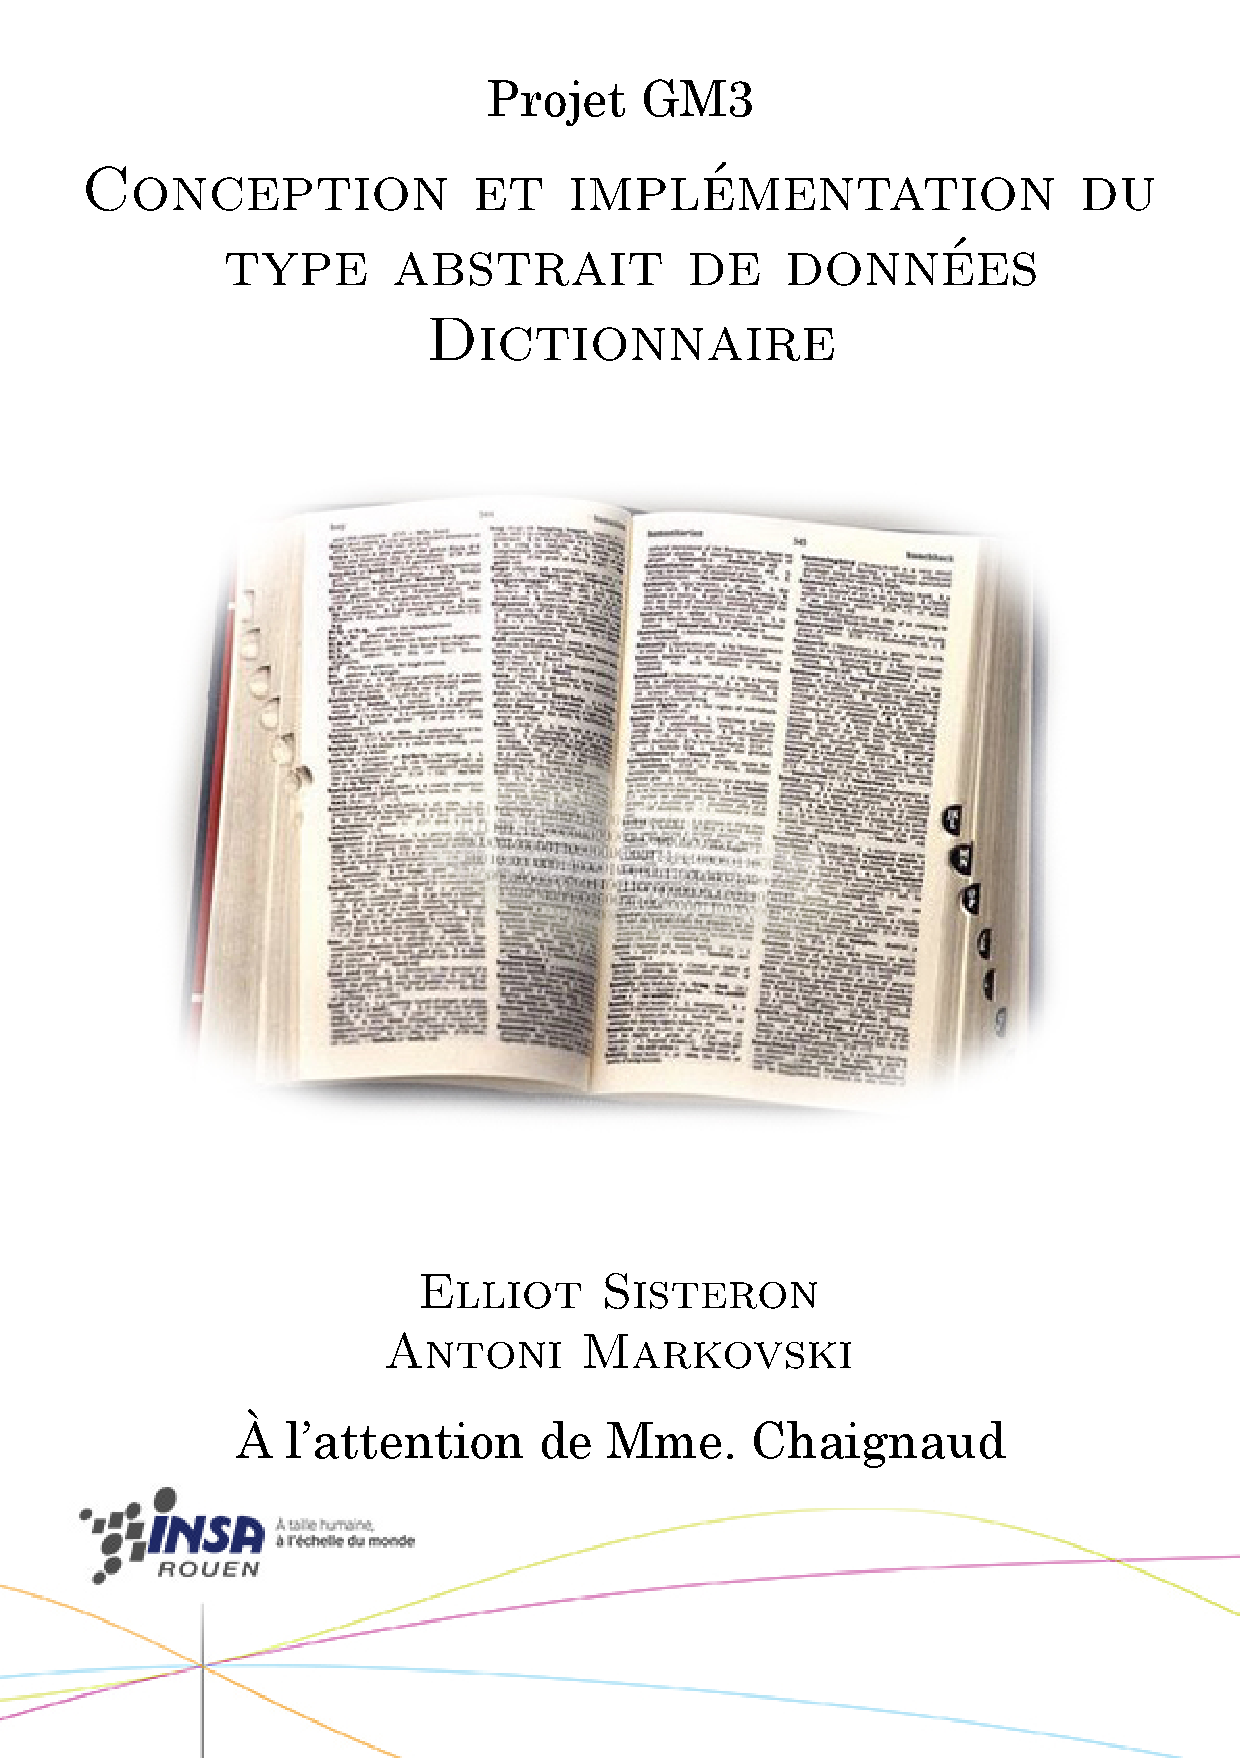
\includepdf{pdf/cover.pdf} % page de garde
	
	\chapter*{Introduction}
	\addcontentsline{toc}{chapter}{Introduction} % ajouter l'introduction au sommaire
		Lorsque l'on veut répertorier un \og grand \fg{} nombre d'informations, il est souvent bien plus pratique de considérer le stockage numérique.
		Pour un dictionnaire français, par exemple, la version papier devient rapidement encombrante (1910 pages de mots et définitions pour \textit{Le petit Larousse}, édition 2012).
		De plus, nous traitons cette information bien plus lentement qu'une machine : la recherche d'un mot dans un dictionnaire papier peut parfois s'avérer laborieuse.
		Il est aussi important de souligner que la modification (insertion/suppression de mots) d'un dictionnaire papier (qui est régi par l'ordre lexicographique) engendre la création d'une multitude d'éditions…
		On comprend alors rapidement l'intérêt de \og numériser \fg{} un tel objet.
		
		Dans ce projet, on cherchera à être capable de manipuler des dictionnaires électroniques de mots avec leurs définitions.
		Pour cela, nous commencerons par définir rigoureusement le type abstrait de données (ou TAD) \textit{Dictionnaire}.
		Puis, nous étudierons la conception du type de données Dictionnaire où nous passerons en revue une interprétation bien précise de ce TAD.
		On débattra alors de son efficacité, sa fiabilité, sa maintenabilité et de sa portabilité.

	\setcounter{tocdepth}{2} % profondeur table des matières
	\tableofcontents % table des matières
	
	\chapter{Le TAD Dictionnaire}
		Dans cette partie, nous allons définir le type abstrait de données \textit{Dictionnaire} pour ensuite essayer de le conceptualiser.

		\section{Présentation du TAD Dictionnaire}
			À première vue, il apparaît qu'un dictionnaire est composé de plusieurs couples (un mot et sa définition).
			Un objet abstrait de type \textit{Dictionnaire} aura donc deux paramètres : \textit{Mot} et \textit{Définition}.
			En tant qu'utilisateur, on arrive bien à percevoir que les opérations suivantes doivent être réalisables :
			\begin{itemize}
				\item Savoir si un mot est présent dans le dictionnaire (en tant qu'\og humain \fg{} : rechercher dans l'index si le mot est présent).
				\item Rechercher une définition à partir d'un mot (en tant qu'\og humain \fg{} : ouvrir le dictionnaire et localiser le mot recherché pour avoir sa définition).
			\end{itemize}
			Mais il faut aussi se placer en tant qu'\og éditeur \fg, d'où la nécessité des opérations :
			\begin{itemize}
				\item Créer un dictionnaire \og vide \fg{} (en tant qu'\og humain \fg{} : aller chez l'imprimeur et demander un livre vierge).
				\item Ajouter un mot avec sa définition dans le dictionnaire, en prenant soin de l'insérer en suivant l'ordre lexicographique (en tant qu'\og humain \fg{} : prendre une plume et écrire le mot avec sa définition au bon endroit, ce qui n'est pas pratique).
				\item Supprimer un mot du dictionnaire (en tant qu'\og humain \fg{} : raturer le mot en question avec sa définition).
			\end{itemize}
			On peut donc proposer le TAD \textit{Dictionnaire} suivant :\\
			\begin{tad}
				\tadNom{Dictionnaire}
				\tadParametres{Mot, Définition}
				\tadDependances{\booleen}
				
				\begin{tadOperations}{Dictionnaire}
					\tadOperation{dictionnaire}{}{\tadUnParam{Dictionnaire}}
					\tadOperation{estPresent}{\tadDeuxParams{Dictionnaire}{Mot}}{\booleen}
					\tadOperationAvecPreconditions{obtenirDefinition}{\tadDeuxParams{Dictionnaire}{Mot}}{Dictionnaire}
					\tadOperation{inserer}{\tadTroisParams{Dictionnaire}{Mot}{Définition}}{\tadUnParam{Dictionnaire}}
					\tadOperation{supprimer}{\tadDeuxParams{Dictionnaire}{Mot}}{\tadUnParam{Dictionnaire}}
				\end{tadOperations}
				
				\begin{tadAxiomes}
					\tadAxiome{inserer(inserer(d, m, def), m, def) = inserer(d, m, def)}
					\tadAxiome{supprimer(supprimer(d, m), m) = supprimer(d, m)}
					\tadAxiome{supprimer(inserer(d, m, def), m) = d}
					\tadAxiome{obtenirDefinition(inserer(d, m, def), m) = def}
					\tadAxiome{obtenirDefinition(supprimer(d, m), m) = creerDefinition()}
					\tadAxiome{estPresent(inserer(d, m, def), m) = Vrai}
					\tadAxiome{non(estPresent(supprimer(d, m), m)) = Vrai}
					\tadAxiome{…}
				\end{tadAxiomes}
			\end{tad}

			On s'intéressera par la suite à une opération de fusion de deux dictionnaires \og compatibles \fg{} (qui, pour un même mot, se réfèrent à la même définition).

		\section{La structure de données choisie}
			On commence par choisir d'implémenter les paramètres de ce TAD (\textit{Mot} et \textit{Définition}) par des chaînes de caractères.
			Dans la suite du projet, on supposera que l'on sait gérer ces chaînes de caractères.
			On pourra donc tester l'égalité de deux chaînes à l'aide des opérateurs $=$ et $\neq$, mais aussi étudier l'ordre lexicographique à l'aide de $<$, $>$, $\leq$, $\geq$.
			De plus, on admettra que l'on peut accéder au $i-$ème caratère d'une chaîne à l'aide de l'opérateur $[\ ]$ (le même que les tableaux).
			Enfin, on supposera que l'on possède une fonction $longueur$ qui renvoie la longueur d'une chaîne passée en paramètre.

			Pour implémenter le TAD \textit{Dictionnaire} en un type de données, on va utiliser une structure de données bien précise :
			une implémentation avec une liste chaînée ordonnée de mots avec leurs définitions (ce qui est un peu lourd en terme de complexité car l'accès à un mot est en $O(n)$). 
			On se propose de diviser cette liste chaînée de couples de mots/définitions en 26 parties dans un tableau indicé par les lettres de l'alphabet.
			Ainsi, la liste chaînée de tous les mots commençant par A (avec leurs définitions) se trouvera dans la case du tableau indicée par le caractère 'A', etc.

			Nous allons conceptualiser en détail cette structure de données.

		\section{Préliminaire : à propos des mots}
			On a vu que l'on pouvait représenter les mots et les définitions du TAD \textit{Dictionnaire} par des chaînes de caractères.
			Toutefois, il nous faudra être prudent en considérant cette représentation pour des mots : par exemple, une chaîne de caractères peut très bien contenir des espaces ou de la ponctuation.
			C'est pour cette raison que l'on se donne la fonction suivante (facilement réalisable…) :\\
			\begin{algorithme}
				\signatureFonction{estUnMot}{ch : \chaine}{\booleen}\\
			\end{algorithme}

			On supposera que l'on a aussi une fonction $maj$ qui mettra en majuscule ASCII un caractère passé en paramètre :\\
			\begin{algorithme}
				\signatureFonction{maj}{c : \caractere}{\caractere}\\
			\end{algorithme}

			Par exemple : 
			\begin{itemize}
				\item maj('b') = 'B'
				\item maj('à') = 'A'
				\item maj('É') = 'E'
				\item maj('L') = 'L'…
			\end{itemize}


	\chapter{Implémentation avec des listes chaînées}
		Dans cette partie, on propose d'implémenter le TAD \textit{Dictionnaire} à l'aide de listes chaînées.

		\section{Conception préliminaire}
			\subsection{Le type Dictionnaire}
				On se donne un type de liste chaînée contenant un mot et sa définition et nous l'appelons ListeChaineeMD (MD pour Mot/Définition) : \\
				\begin{algorithme}
					\begin{enregistrement}{Noeud}
						\champEnregistrement{mot}{\chaine}
						\champEnregistrement{definition}{\chaine}
						\champEnregistrement{suivant}{\typePointeur{Noeud}}
					\end{enregistrement}\\
					\type{ListeChaineeMD}{\typePointeur{Noeud}}\\
				\end{algorithme}

				On propose alors le type de données Dictionnaire suivant :\\
				\begin{algorithme}
					\type{Dictionnaire}{\tableauUneDimension{'A'..'Z'}{de }{ListeChaineeMD}}\\
				\end{algorithme}

				On peut se représenter, sur un exemple, le type Dictionnaire par le schéma suivant :
				\begin{figure}[!ht]
				\centering
  					\includegraphics[scale=0.45]{liste.png}
  					\caption{Une implémentation du TAD \textit{Dictionnaire} avec des listes chaînées et un tableau} 
				\end{figure}


				\subsection{Les signatures des opérations}
					On se donne les signatures des opérations du type de données Dictionnaire suivantes :\\
					\begin{algorithme}
						\signatureFonction{creerDictionnaire}{}{Dictionnaire}
						\signatureFonction{estPresent}{d : Dictionnaire, m : \chaine}{\booleen}
						\signatureFonction{obtenirDefinition}{d : Dictionnaire, m : \chaine}{\chaine}
						\signatureProcedureAvecPreconditions{inserer}{\paramEntreeSortie{d : Dictionnaire}, \paramEntree{m, def : \chaine}}{estUnMot(m)}
						\signatureProcedure{supprimer}{\paramEntreeSortie{d : Dictionnaire}, \paramEntree{m : \chaine}}
						\signatureFonction{fusionner}{d1, d2 : Dictionnaire}{Dictionnaire}
					\end{algorithme}

		\section{Conception détaillée}
			\subsection{La création de dictionnaire}
				Cet algorithme va nous permettre de créer un dictionnaire \og vide \fg{}.
				Pour cela, il est nécessaire d'initialiser chacune des listes chaînées à NIL.
				\begin{figure}[!ht]
				\centering
  					\includegraphics[scale=0.45]{creerDictionnaire.png}
  					\caption{Un schéma pour mieux comprendre le fonctionnement de $creerDictionnaire$} 
				\end{figure}

				\begin{algorithme}
					\fonction{creerDictionnaire}{}{Dictionnaire}
					{res : Dictionnaire, i : \caractere}{
						\pour{i}{'A'}{'Z'}{}{
							\affecter{res[i]}{NIL}
						}
						\retourner{(res)}
					}
				\end{algorithme}
			\subsection{La présence d'un mot dans le dictionnaire}
				On veut tester la présence d'un mot $m$ dans un dictionnaire $d$.
				Autrement dit, on va vérifier que le mot se trouve dans la liste chaînée correspondant à sa première lettre.
				La première chose à faire est donc de se positionner dans la \og bonne \fg{} liste chaînée.
				\begin{figure}[!ht]
				\centering
  					\includegraphics[scale=0.45]{estPresent1.png}
  					\caption{Dans cet exemple, le mot recherché commence par la lettre A} 
				\end{figure}
				\newpage

				Pour cela, on transforme la première lettre du mot (c'est-à-dire m[1]) en majuscule pour avoir l'indice correspondant.
				On se positionne donc dans la case $d[maj(m[1])]$ du tableau.
				À ce stade, on positionne un curseur sur la liste pour pouvoir la parcourir.
				\begin{figure}[!ht]
				\centering
  					\includegraphics[scale=0.45]{estPresent2.png}
  					\caption{On s'apprête à parcourir la liste chaînée} 
				\end{figure}


				Pour optimiser un peu la recherche du mot $m$, on utilise le fait que la liste que l'on va parcourir est ordonnée.
				Autrement dit, on se positionnera sur le premier mot supérieur ou égal à $m$ plutôt que de parcourir toute la liste jusqu'à ce qu'on le trouve.
				Si ce mot est égal à $m$, alors on aura trouvé $m$. 
				\begin{figure}[!ht]
				\centering
  					\includegraphics[scale=0.45]{estPresent3.png}
  					\caption{Dans cet exemple on a trouvé $m$} 
				\end{figure}
				\newpage

				Sinon, $m$ n'est pas dans la liste car tous les mots suivants seront supérieurs strictement à $m$ (du fait que la liste soit ordonnée).
				\begin{figure}[!ht]
				\centering
  					\includegraphics[scale=0.45]{estPresent4.png}
  					\caption{Dans cet exemple, $m$ n'est pas dans la liste} 
				\end{figure}

				Bien sûr, il existera un cas où le parcours sera entièrement réalisé : celui où tous les mots se trouvant dans la liste sont inférieurs strictement à $m$.
				\begin{figure}[!ht]
				\centering
  					\includegraphics[scale=0.45]{estPresent5.png}
  					\caption{Le pire des cas} 
				\end{figure}

				Résumons tout cela.
				Tant que le que le curseur n'est pas arrivé au bout ou que le mot du curseur est inférieur strictement au mot recherché, on avance.
				Si le curseur est arrivé au bout, alors le mot n'est pas présent.
				Si le curseur n'est pas arrivé à la fin de la liste, alors :
				\begin{itemize}
					\item S'il se trouve sur l'élément recherché, alors l'élément en question est bien présent.
					\item Par contre, si le mot sur lequel il est positionné n'est pas le mot recherché, alors le mot ne se trouve pas dans la liste (car celle-ci est ordonnée et les éléments suivants sont donc strictement supérieurs).
				\end{itemize}

				On en déduit donc l'algorithme suivant :\\
				\begin{algorithme}
					\fonction{estPresent}{d : Dictionnaire, m : \chaine}{\booleen}
					{curseur : ListeChaineeMD}{
						\affecter{curseur}{d[maj(m[1])]}
						\tantque{((curseur $\neq$ NIL) et (\pointeur{curseur}.mot $<$ m))}{
							\affecter{curseur}{\pointeur{curseur}.suivant}
						}
						\retourner{((curseur $\neq$ NIL) et (\pointeur{curseur}.mot $=$ m))}
					}
				\end{algorithme}

			\subsection{Récupérer une définition}
				On cherche à récupérer la définition d'un mot $m$ qui est dans un dictionnaire $d$.
				Pour cela, on se place encore dans la bonne case du tableau, et on parcoure la liste chaînée pour le retrouver.
				Il s'agit quasiment du même algorithme que le précédent sauf que, une fois positionné sur le bon élément de la liste, on retourne la définition.
				Si le mot n'a pas été trouvé, on retourne une chaîne nulle.\\
				\begin{algorithme}
					\fonction{obtenirDefinition}{d : Dictionnaire, m : \chaine}{\chaine}
					{curseur : ListeChaineeMD, res : \chaine}{
						\affecter{res}{""}
						\affecter{curseur}{d[maj(m[1])]}
						\tantque{((curseur $\neq$ NIL) et (\pointeur{curseur}.mot $<$ m))}{
							\affecter{curseur}{\pointeur{curseur}.suivant}
						}
						\sialors{((curseur $\neq$ NIL) et (\pointeur{curseur}.mot $=$ m))}{
							\affecter{res}{\pointeur{curseur}.definition}
						}
						\retourner{(res)}
					}
				\end{algorithme}

			\subsection{Lois de composition externes}
				On a deux lois de composition externes sur un dictionnaire : l'insertion d'un mot ou la suppression d'un mot.

				\subsubsection{Insertion d'un mot avec sa définition}
					On cherche ici à insérer un mot $m$ avec sa définition $def$ dans un dictionnaire $d$.
					On récupère, là encore, la liste chaînée à laquelle $m$ appartient dans le dictionnaire $d$ et on veut l'insérer au bon endroit dans cette liste.
					On commence par positionner un curseur sur cette liste.

					On distingue tout d'abord deux cas particuliers.
					Le cas où la liste dans laquelle on va insérer $m$ est vide ou encore le cas où le premier mot de la liste est supérieur strictement à $m$.
					Cela signifie que nous allons devoir insérer $m$ et sa définition en tête de liste.

					Pour cela, on commence par allouer un espace mémoire de la taille de \textit{Noeud} que l'on fait pointer sur une variable $tmp$, dans lequel on copie $m$ et $def$.
					Ensuite, on fait pointer la case du dictionnaire $d[maj(m[1])]$ sur $tmp$ et enfin on fait pointer le champ suivant de $tmp$ sur le curseur.
					\begin{figure}[!ht]
					\centering
  						\includegraphics[scale=0.45]{inserer1.png}
  						\caption{Les deux cas particuliers pour l'insertion en tête de liste} 
					\end{figure}

					On distingue aussi le cas d'insertion en fin de liste, c'est à dire le cas où tous les mots de la liste sont inférieurs strictement à $m$.
					On positionne le curseur juste avant d'arriver en fin de liste (c'est-à-dire de telle manière que le champ suivant du curseur pointe sur NIL).
					Dès lors, on alloue encore un espace mémoire $tmp$, on fait pointer le champ suivant de $tmp$ sur le champ suivant du curseur (c'est-à-dire  liste sur NIL), puis l'on fait pointer le champ suivant du curseur sur $tmp$.
					\begin{figure}[!ht]
					\centering
  						\includegraphics[scale=0.45]{inserer2.png}
  						\caption{Le cas particulier d'insertion en fin de liste} 
					\end{figure}

					Pour le cas général, on va positionner le curseur sur un élément inférieur strictement à $m$ mais aussi juste avant un élément supérieur strictement à $m$ (on veut \og intercaler \fg{} $m$ de cette manière pour garder une liste ordonnée).
					Il s'agit alors de la même insertion que l'insertion en fin de liste.
					\begin{figure}[!ht]
					\centering
  						\includegraphics[scale=0.45]{inserer3.png}
  						\caption{Le cas général} 
					\end{figure}\\

					Il ne faut pas oublier le cas particulier où le mot se trouve déjà dans la liste chaînée.
					Il nous faudra donc éviter de l'insérer une deuxième fois dans la liste en s'arrêtant dès qu'on le rencontre.
					\begin{figure}[!ht]
					\centering
  						\includegraphics[scale=0.45]{inserer4.png}
  						\caption{On ne fait rien lorsque le mot est déjà dans la liste} 
					\end{figure}
				
					Résumons-nous.
					On positionne un curseur.
					Si le curseur pointe sur NIL ou si le mot du curseur est supérieur strictement à $m$, alors on insère en tête.
					Sinon, si le curseur n'est pas positionné sur $m$, tant que le champ suivant du curseur ne pointe pas sur NIL et que le mot du champ suivant du curseur est inférieur strictement à $m$, on avance.
					Si l'on a arrêté d'avancer parce que le champ suivant du curseur pointait sur NIL, alors on insère en fin de liste.
					Sinon c'est que l'on s'est arrété parce que le mot du champ suivant du curseur était supérieur ou égal à $m$.
					S'il n'est pas égal à $m$, on peut insérer (et c'est la même insertion qu'en fin de liste).

					D'où l'algorithme : \\
					\begin{algorithme}
						\procedureAvecPreconditions{inserer}{\paramEntreeSortie{d : Dictionnaire}, \paramEntree{m, def : \chaine}}{estUnMot(m)}
						{tmp, curseur : ListeChaineeMD}{
							\affecter{curseur}{d[maj(m[1])]}
							\sialorssinon{((curseur $=$ NIL) ou (\pointeur{curseur}.mot $>$ m))}{
								\affecter{tmp}{\allouer{Noeud}}					
								\affecter{\pointeur{tmp}.mot}{m}
								\affecter{\pointeur{tmp}.definition}{def}
								\affecter{d[maj(m[1])]}{tmp}
								\affecter{\pointeur{tmp}.suivant}{curseur}
							}{
								\sialors{(\pointeur{curseur}.mot $\neq$ m)}{
									\tantque{((\pointeur{curseur}.suivant $\neq$ NIL) et (\pointeur{\pointeur{curseur}.suivant}.mot $<$ m))}{
										\affecter{curseur}{\pointeur{curseur}.suivant}
									}
									\sialors{((\pointeur{curseur}.suivant $=$ NIL) ou (\pointeur{\pointeur{curseur}.suivant}.mot $\neq$ m))}{
										\affecter{tmp}{\allouer{Noeud}}					
										\affecter{\pointeur{tmp}.mot}{m}
										\affecter{\pointeur{tmp}.definition}{def}
										\affecter{\pointeur{tmp}.suivant}{\pointeur{curseur}.suivant}
										\affecter{\pointeur{curseur}.suivant}{tmp}
									}
								}
							}
						}
					\end{algorithme}

				\subsubsection{Suppression d'un mot et sa définition}
					On cherche maintenant à supprimer un mot $m$ dans un dictionnaire $d$.
					Là encore, on commence par positionner un curseur sur la liste qui est susceptible de contenir $m$.
					On va parcourir cette liste de la même manière que pour l'insertion, et on libèrera l'espace mémoire pris par le mot et sa définition une fois celui-ci trouvé.

					Tout d'abord, si la liste est vide (c'est-à-dire si le curseur est égal à NIL), on ne fait évidemment rien.
					Si la liste commence par $m$, on procédera en faisant pointer la case du dictionnaire $d[maj(m[1])]$ sur l'élément suivant du curseur, puis on libérera le curseur (suppression en tête).
					\begin{figure}[!ht]
					\centering
  						\includegraphics[scale=0.45]{supprimer1.png}
  						\caption{Le cas particulier de suppression en tête} 
					\end{figure}
					\newpage

					Concernant le cas général, il s'agit du même principe que pour l'insertion : on avance le curseur jusqu'à ce que son champ suivant pointe sur le \textit{Noeud} contenant $m$.
					On utilise alors une variable $tmp$ que l'on fait pointer sur le champ suivant du curseur.
					Dès lors, il suffit de faire pointer le curseur sur le champ suivant du champ suivant du curseur (c'est-à-dire sur le champ suivant de $tmp$), puis de libérer l'espace mémoire $tmp$.
					\begin{figure}[!ht]
					\centering
  						\includegraphics[scale=0.45]{supprimer2.png}
  						\caption{Le cas général} 
					\end{figure}

					Il faudra aussi faire attention à un autre cas particulier : celui où le mot $m$ n'est pas présent dans la liste.
					Il sera donc nécessaire de tester cette éventualité.
					\begin{figure}[!ht]
					\centering
  						\includegraphics[scale=0.45]{supprimer3.png}
  						\caption{Lorsque $m$ n'est pas dans la liste, on ne fait rien} 
					\end{figure}

					Résumons cela.
					On positionne un curseur.
					Tout d'abord, si le curseur pointe sur NIL, on ne fait rien. 
					Maintenant, si le mot du curseur est $m$, on supprime la tête de liste.
					Sinon, tant que le champ suivant du curseur ne pointe pas sur NIL et que le mot du champ suivant du curseur est inférieur strictement à $m$, on avance.
					Si l'on s'est arrêté parce que le mot du champ suivant du curseur est égal à $m$, alors on supprime le \textit{Noeud} contenant $m$.

					On peut donc en déduire l'algorithme :\\
					\begin{algorithme}
						\procedure{supprimer}{\paramEntreeSortie{d : Dictionnaire}, \paramEntree{m : \chaine}}
						{tmp, curseur : ListeChaineeMD}{
							\affecter{curseur}{d[maj(m[1])]}
							\sialors{(curseur $\neq$ NIL)}{
								\sialorssinon{(\pointeur{curseur}.mot $=$ m)}{
									\affecter{d[maj(m[1])]}{\pointeur{curseur}.suivant}
									\item{\textbf{libérer}(curseur)}
								}{
									\tantque{((\pointeur{curseur}.suivant $\neq$ NIL) et (\pointeur{\pointeur{curseur}.suivant}.mot $<$ m))}{
										\affecter{curseur}{\pointeur{curseur}.suivant}
									}
									\sialors{((\pointeur{curseur}.suivant $\neq$ NIL) et (\pointeur{\pointeur{curseur}.suivant}.mot $=$ m))}{
										\affecter{tmp}{\pointeur{curseur}.suivant}
										\affecter{\pointeur{curseur}.suivant}{\pointeur{tmp}.suivant}
										\item{\textbf{libérer}(tmp)}
									}
								}
							}
						}
					\end{algorithme}
			
			\subsection{La loi de composition interne fusionner}
				On cherche ici à fusionner deux dictionnaires \og compatibles \fg{} en prenant soin de ne pas laisser de doublons.
				La première approche (la plus évidente), consiste à insérer tous les éléments des deux dictionnaires dans un seul dictionnaire.
				On se donne donc une variable $res$ de type Dictionnaire.
				Pour chaque liste des deux dictionnaires, on insère tous les éléments de ces listes dans $res$.

				Il nous faut ici créer une procédure d'insertion d'une ListeChaineeMD dans un dictionnaire :\\
				\begin{algorithme}
					\procedure{ajouterListeMD}{\paramEntreeSortie{d : Dictionnaire}, \paramEntree{l : ListeChaineeMD}}
					{}{
						\tantque{(l $\neq$ NIL)}{
							\item{inserer(d, \pointeur{l}.mot, \pointeur{l}.definition)}
							\affecter{l}{\pointeur{l}.suivant}
						}
					}\\
				\end{algorithme}

				La fonction fusionner devient alors :\\
				\begin{algorithme}
					\fonction{fusionner}{d1, d2 : Dictionnaire}{Dictionnaire}
					{res : Dictionnaire, i : \caractere}{
						\affecter{res}{creerDictionnaire()}
						\pour{i}{'A'}{'Z'}{}{
							\item{ajouterListeMD(res, d1[i])}
							\item{ajouterListeMD(res, d2[i])}
						}
						\retourner{(res)}						
					}\\
				\end{algorithme}

				On remarque ici que la complexité de la procédure \textit{ajouterListeMD} est très élevée : en effet, à chaque itération de la boucle \textit{tant que} on utilise l'opération $inserer$ qui est en O(n).
				Autrement dit, comme la boucle \textit{tant que} parcoure toute la liste chaînée, on est globalement en O($n^2$), ce qui est relativement mauvais.
				On se propose donc de travailler directement sur les listes sans passer par l'opération $inserer$, pour retrouver une complexité en $O(n)$.

				Nous allons créer une fonction de fusion de deux ListeChaineeMD que nous appliquerons aux listes des deux dictionnaires à fusionner.
				On se donne donc deux ListeChaineeMD $l1$ et $l2$ et une variable $res$ pour stocker le résultat.
				On place des curseurs : $curseur1$ sur $l1$, $curseur2$ sur $l2$ et $curseur$ sur $res$.
				On allouera au fur et à mesure un espace mémoire $tmp$ dans lequel on chargera le couple mot/définition en cours de traitement, que l'on ira chaîner sur le $curseur$ de $res$ que l'on fera ensuite avancer.
				
				On commence par remarquer un premier cas particulier : celui où $l1$ et $l2$ sont égales à NIL.
				Le résultat devra donc être NIL.	
				\begin{figure}[!ht]
				\centering
  					\includegraphics[scale=0.39]{fusionner1.png}
  					\caption{Un premier cas particulier} 
				\end{figure}

				Ensuite, il faut aussi traiter le cas où seulement l'une des deux listes est remplie.
				Si $l1$ est remplie et pas $l2$ par exemple, il suffit d'allouer un par un les éléments de $l1$ dans $res$, en utilisant le $curseur1$ pour se balader sur la liste chaînée.
				\begin{figure}[!ht]
				\centering
  					\includegraphics[scale=0.39]{fusionner2.png}
  					\caption{Un second cas particulier} 
				\end{figure}

				Si les deux listes sont remplies, alors il faudra comparer leurs éléments au fur et à mesure pour avoir une liste $res$ ordonnée.
				Si l'élément de $l1$ est inférieur à celui de $l2$, il faudra le mettre avant dans $res$ puis avancer le $curseur1$.
				Si le mot rencontré après dans $l1$ est supérieur à celui de $l2$, alors il faudra copier dans $res$ le mot de $l2$ et faire avancer le $curseur2$…
				Ainsi de suite jusqu'à ce que l'on arrive à un des deux cas terminaux précédents (une des deux listes (ou les deux) est égale à NIL).
				\begin{figure}[!ht]
				\centering
  					\includegraphics[scale=0.39]{fusionner3.png}
  					\caption{Le cas général} 
				\end{figure}

				Attention, il nous faudra aussi prendre en compte le cas où les deux éléments comparés sont égaux : pour ne pas le copier deux fois à la suite, on déplacera $curseur1$ et $curseur2$ en même temps.\\

				\begin{algorithme}
					\fonction{fusionnerListeMD}{l1, l2 : ListeChaineeMD}{ListeChaineeMD}
					{res, tmp, curseur : ListeChaineeMD}{
						\affecter{res}{NIL}
						\affecter{curseur1}{l1}
						\affecter{curseur2}{l2}
						\tantque{(curseur1 $\neq$ NIL) et (curseur2 $\neq$ NIL)}{
							\affecter{tmp}{\allouer{Noeud}}
							\sialorssinon{(\pointeur{curseur1}.mot $\leq$ \pointeur{curseur2}.mot)}{
									\sialors{(\pointeur{curseur1}.mot $=$ \pointeur{curseur2}.mot)}{
										\affecter{curseur2}{\pointeur{curseur2}.suivant}
									}
									\affecter{\pointeur{tmp}.mot}{\pointeur{curseur1}.mot}
									\affecter{\pointeur{tmp}.definition}{\pointeur{curseur1}.definition}
									\affecter{curseur1}{\pointeur{curseur1}.suivant}
							}{
									\affecter{\pointeur{tmp}.mot}{\pointeur{curseur2}.mot}
									\affecter{\pointeur{tmp}.definition}{\pointeur{curseur2}.definition}
									\affecter{curseur2}{\pointeur{curseur2}.suivant}
							}
							\sialorssinon{(res = NIL)}{
								\affecter{res}{tmp}
								\affecter{curseur}{tmp}
							}{
								\affecter{\pointeur{curseur}.suivant}{tmp}
								\affecter{curseur}{tmp}
							}
						}	
						\sialorssinon{(curseur1 $=$ NIL)}{
							\tantque{(curseur2 $\neq$ NIL)}{
								\affecter{tmp}{\allouer{Noeud}}
									\affecter{\pointeur{tmp}.mot}{\pointeur{curseur2}.mot}
									\affecter{\pointeur{tmp}.definition}{\pointeur{curseur2}.definition}
									\sialorssinon{(res = NIL)}{
										\affecter{res}{tmp}
										\affecter{curseur}{tmp}
									}{
										\affecter{\pointeur{curseur}.suivant}{tmp}
										\affecter{curseur}{tmp}
									}
							}
						}{
							\tantque{(curseur1 $\neq$ NIL)}{
								\affecter{tmp}{\allouer{Noeud}}
									\affecter{\pointeur{tmp}.mot}{\pointeur{curseur1}.mot}
									\affecter{\pointeur{tmp}.definition}{\pointeur{curseur1}.definition}
									\sialorssinon{(res = NIL)}{
										\affecter{res}{tmp}
										\affecter{curseur}{tmp}
									}{
										\affecter{\pointeur{curseur}.suivant}{tmp}
										\affecter{curseur}{tmp}
									}
							}
						}
						\sialors{(res $\neq$ NIL)}{
							\affecter{\pointeur{curseur}.suivant}{NIL}
						}
						\retourner{(res)}	
					}\\
				\end{algorithme}

				\begin{algorithme}
					\fonction{fusionner}{d1, d2 : Dictionnaire}{Dictionnaire}
					{res : Dictionnaire, i : \caractere}{
						\affecter{res}{creerDictionnaire()}
						\pour{i}{'A'}{'Z'}{}{
							\affecter{res[i]}{fusionnerListeMD(d1[i], d2[i])}
						}
						\retourner{(res)}						
					}\\
				\end{algorithme}


		\section{Complexité}
			Avec les listes, on a les complexités suivantes :
			\begin{figure}[!ht]
				\begin{tabular}{|*{6}{c|}}
    				\hline
    				creerDictionnaire & estPresent & obtenirDefinition & inserer & supprimer & fusionner \\
    				\hline
    				$\Omega$(1) & $\Omega$(1) & $\Omega$(1) & $\Omega$(1) & $\Omega$(1) & $\Omega$(1) \\
    				\hline
    				O(1) & O(n) & O(n) & O(n) & O(n) & O(n) \\
    				\hline
				\end{tabular}
				\caption{Complexité des opérations}
			\end{figure}

			On ne parle pas de la complexité moyenne $\Theta$ (trop compliquée à calculer).
			Toutefois, on peut noter que l'on s'est arrangé pour que celle-ci soit relativement faible (en utilisant notamment le fait que la liste soit ordonnée).

		\section{Bilan}
			Globalement, cette structure de donnée fonctionne parfaitement et reste relativement simple à manipuler.
			Toutefois, la complexité des opérations se révèle assez mauvaise (dans le pire des cas).
			Sur un appareil limité en mémoire vive et en \og puissance brute \fg{} (on pourrait imaginer un petit appareil éléctronique faisant office de dictionnaire), on atteindrait rapidement les limites de cette structure de donnée.

		%\section{Complexité}
		%\section{Bilan}

	%\chapter{Implémentation avec une table de hashage}
	%	Quatrième partie
	%	\section{Présentation}
	%	\section{Conception}
	%	\section{Complexité}
	%	\section{Dévellopement}
	%	\section{Bilan}

	%\chapter{Réalisation d'un programme C}

	
	\chapter*{Conclusion}
	\addcontentsline{toc}{chapter}{Conclusion} % ajouter la conclusion au sommaire
		Ce projet, d'une durée relativement limitée, nous aura néanmoins enseigné de nombreuses choses :
		\begin{itemize}
			\item Une meilleur compréhension de la notion de type abstrait de données.
			\item Une maîtrise plus poussée des listes chaînées, une plus grande maitrise du cours.
			\item De nouvelles connaissances suites aux recherches que nous avons réalisées dans le but de trouver des structures de données plus efficaces.
			\item Une opportunité pour nous perfectionner en langage C en implémentant les algorithmes de ce projet pour s'assurer de leur bon fonctionnement.
		\end{itemize}

		On aura ainsi pu mieux saisir l'importance (et même la nécessité) de la conception préliminaire et détaillée avant le dévellopement de n'importe quelle structure de données informatique.


	\appendix
	\addtocontents{toc}{\protect\setcounter{tocdepth}{0}} % profondeur table des matières annexes

	%\chapter{Afficher un dictionnaire}
	%	Première annexe
	
	%\chapter{Lecture et écriture de dictionnaire avec des fichiers}
	%	Deuxième annexe

	
	%\chapter{Troisième annexe}
	%	Troisième annexe
	%	\lstset{language=C,
	%		inputencoding=utf8/latin1
	%		}

	%	\section{Les headers}
	%		\subsection{IHM}
	%			Fichier : IHM.h
	
	%			\lstinputlisting{src/IHM.h}
	%		
	%		\subsection{Simulation}
	%			Fichier : simulation.h
	
	%			\lstinputlisting{src/simulation.h}
	
	%	\section{Programme principal}
	%		Fichier : main.c
	
	%		\lstinputlisting{src/main.c}
	
	%	\section{Le makefile}
	%		Fichier : Makefile
	%		\lstset{language=make} 
	%	
	%		\lstinputlisting{src/Makefile}
	
	\begin{thebibliography}{9}
	\addcontentsline{toc}{chapter}{Bibliographie} % ajouter la bibliographie au sommaire
	
		\bibitem{Cours 01}
			\emph{Nathalie Chaignaud},
			\textit{Algorithmes et structures de données},
			Institut National des Sciences Appliquées de Rouen, département GM, 2013.

		\bibitem{Cours 02}
			\emph{Nicolas Delestre},
			\textit{Algorithmique et base de la programmation},
			Institut National des Sciences Appliquées de Rouen, département ASI, 2013.
	
	\end{thebibliography}


\end{document} % fin du document
